\newpage
\section{CAN-Transceiver}
\label{sec:CAN-Tranceiver}
The CAN-transceiver is in place to ensure a proper transmission of the CAN signal. Even though the microcrontroller, used as MCU, contains a CAN controller it is still needed to implement a CAN transceiver, according to the protocol as seen on the figure \vref{CAN_Network}.

\begin{figure}[H]
	\centering
	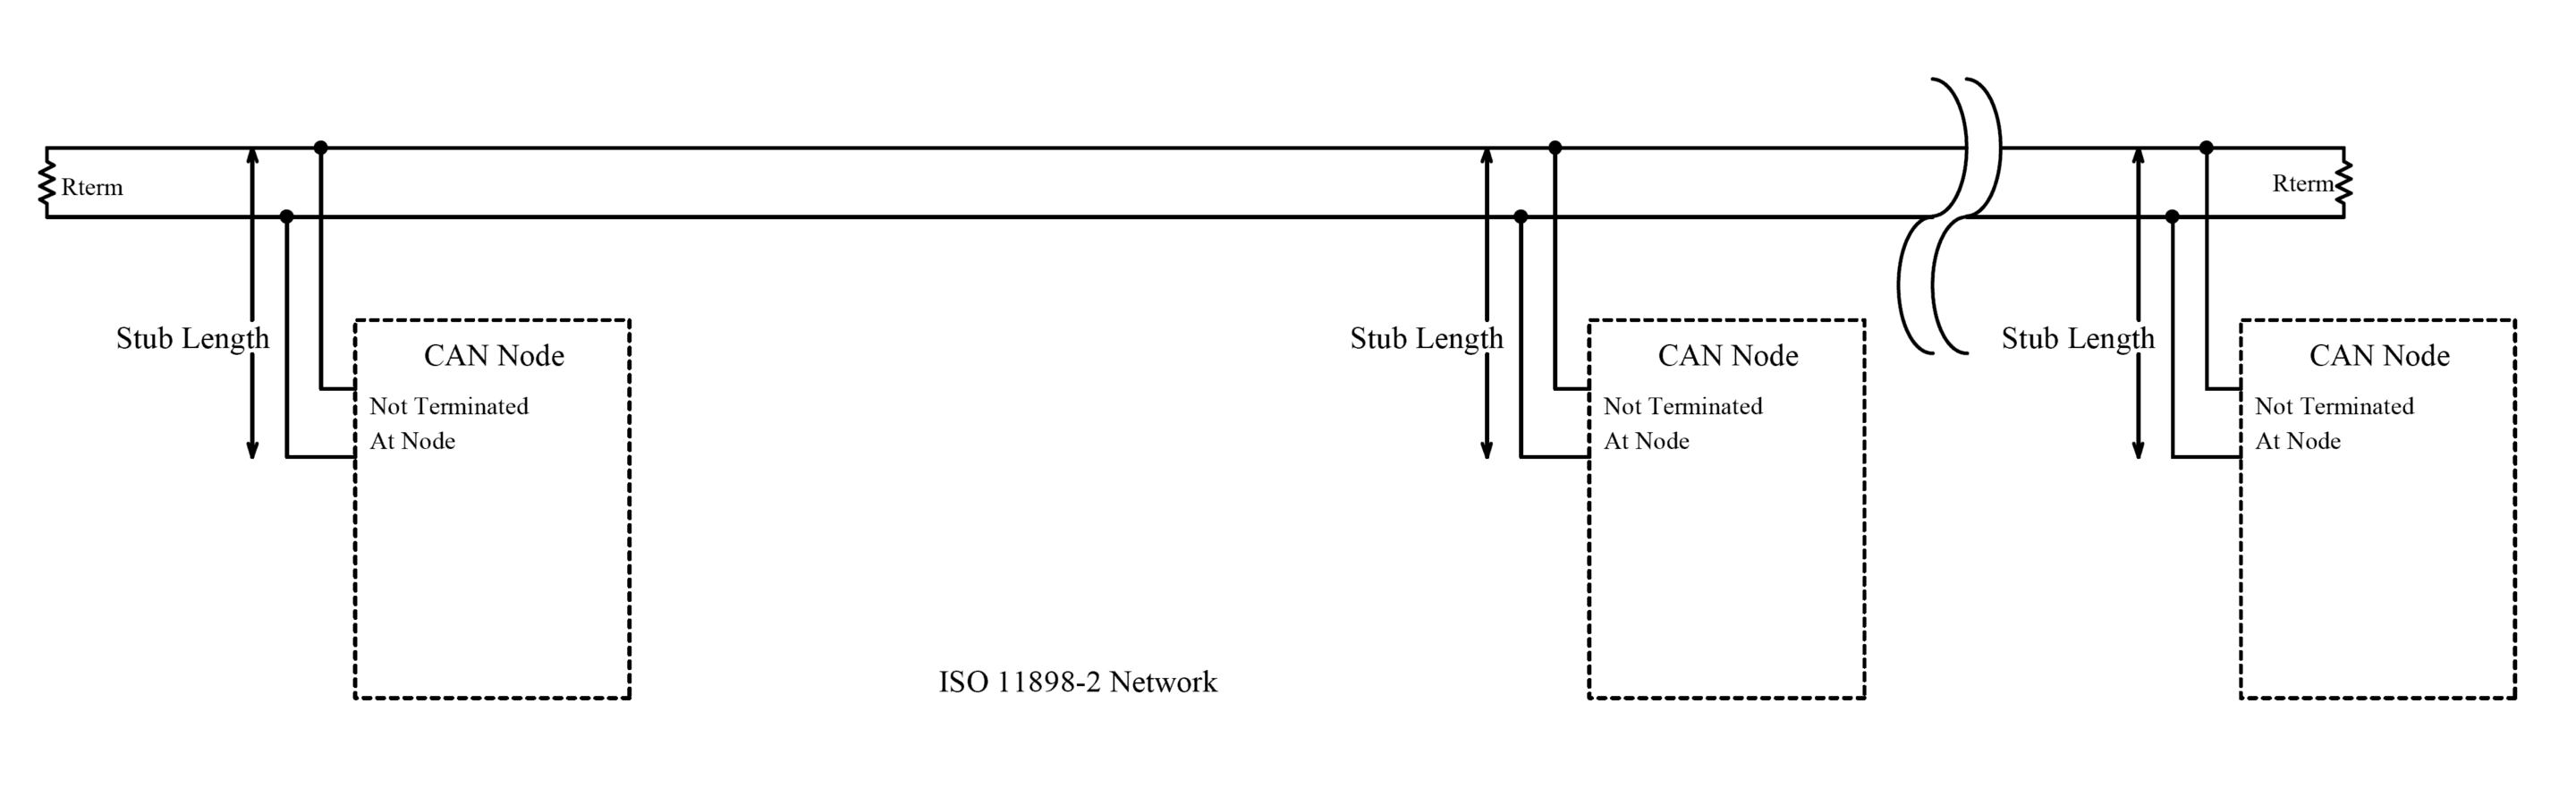
\includegraphics[width=0.7\linewidth]{Hardware/Pictures/CAN_Network}
	\caption{CAN Network overview}
	\label{fig:CAN_Network}
\end{figure}


The CAN bus is used to communicate with BMS and a computer that can be connected to this bus. 

The CAN protocol is implemented, as a result of the BMS in use. On BMS there is implemented a CAN connection and therefore CAN is the obvious choice.    

\subsection{Design}
There exists numerous CAN transceiver packages that can be used for this specific purpose. The specific transceiver at use in this design is SN65HVD1040 \cite{CAN}. This CAN transceiver is chosen for its extremely low power consumption. 

The design for the transceiver can be seen on figure \vref{fig:CAN_hw}. This design is done according to the datasheet. The pin STB is being pulled up with a strong pull up resistor. There is a decoupling capacitor connected on the supply line, as there can occur some relatively large currents as it is a digital circuit. 

\begin{figure}[H]
	\centering
	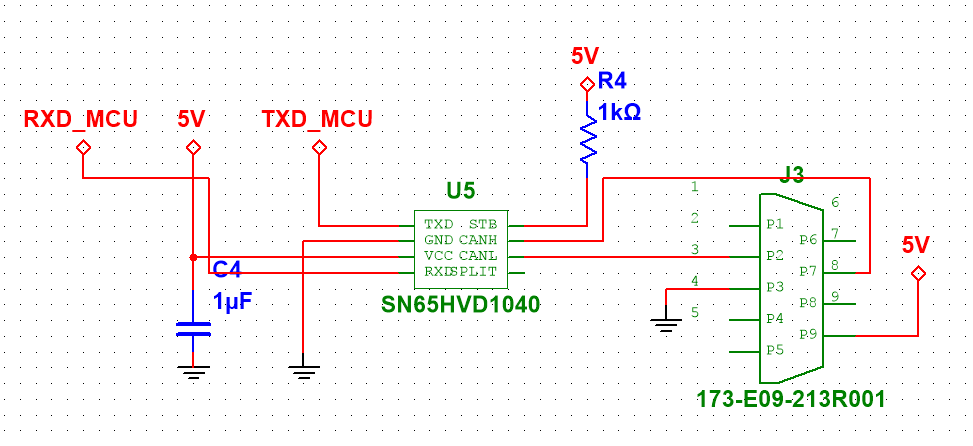
\includegraphics[width=0.7\linewidth]{Hardware/Pictures/CAN_transceiver}
	\caption{CAN transceiver overview}
	\label{fig:CAN_hw}
\end{figure}

\subsection{Implementation}
The implementation is done via a SMD component. Furthermore it is connected to a DSUB9 connector that is used for communication with other systems. The DSUB9 connector is chosen as its counterpart on BMS also uses this connection. The pin-outs are implemented according to the following:

	\begin{itemize}
		\item Pin 2: CAN-low (CAN-)
		\item Pin 3: Ground
		\item Pin 7: CAN-high (CAN+)
		\item Pin 9: Power (5V here)
	\end{itemize} \cite{CAN-Connection}

\subsection{Unity test}
At hand-in this module was not tested. The test can first be done when everything else is up and running as this requires a working PSoC and BMS for it to be properly and thoroughly tested. This is because the rather high complexity of the CAN protocol. 